\unnumberedSection[tradeoffPoints]{Tradeoff Points}

\begin{description}[style=nextline]
  \item[T1\label{t1}] State resynchronisation will have a negative effect on performance, but positive effect on availability
    \vspace{\baselineskip}
    \newline
    Having a state resynchronisation will be beneficial for the availability since it will provide a protocol to recover in case of fault if one of the players do not receive one or many messages and get out of sync. Recovering from this situation may however be processing expensive since a negotiation between all players must be performed in order to determine on which to agreed on and to perform the transfert of the necessary information to all the unsynchronized nodes.

  \item[T2\label{t2}] Template Method Pattern will have negative effect on modifiability, but positive effect on modifiability
    \vspace{\baselineskip}
    \newline
    As surprising as it can be, the evaluation team decided to classify the usage of the Template Method pattern as a tradeoff since we do not consider the this will help achieve the kind of modifiability required by the game dynamic.
    \newline
    \vspace{\baselineskip}
    The Template Method pattern is really useful when we want to make a basic algorithm more flexible. This will usually be necessary when we want to create an interface having different options for transforming and/or interpreting the inputs. If we push it to the limit, we could simply describe the Template Method pattern as the application of polymorphism to procedural code generation. \cite{wiki:templateMethod}
    \newline
    \vspace{\baselineskip}
    However, the kind of modifiability that we are seeking for is much more related to the object behavior itself more than the different subprocesses that we will have to be run to achieve a given result. Using the Template Method pattern may even introduce some undesirable constraints into the design.
    \newline
    \vspace{\baselineskip}
    A better pattern to be used considering the game concept would be the composite pattern where a given interface has to be implemented by the whole class hierarchy which allows us to solve recursive problem such as the construction of a castle and other game elements. The main idea behind the composite pattern is that every object can become a combinaison of sub-object and every time a given method will be called, the main object will simply recursively call the same method over all the objects that he is composed of. Based on this idea, we could then define the castle as a composition of basic shape of blocks. \cite{wiki:composite}
    \begin{center}
      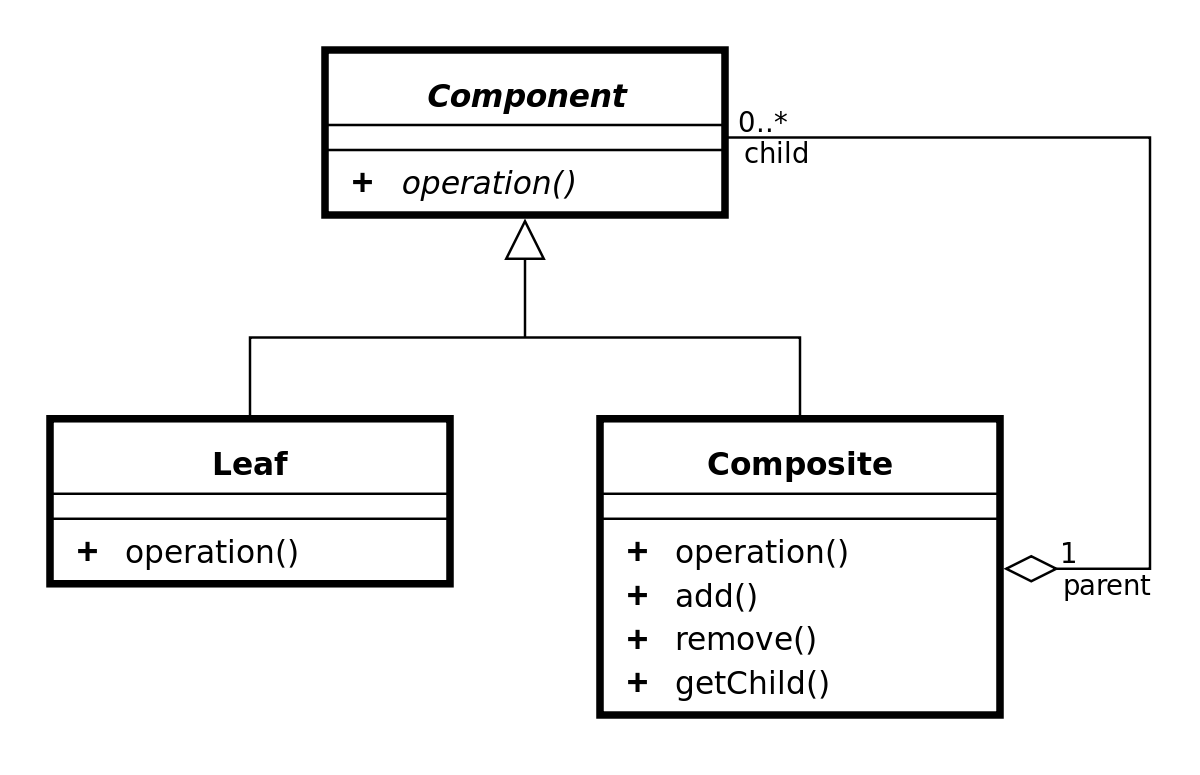
\includegraphics[width=\textwidth,height=0.25\textheight,keepaspectratio]{compositePatternClassDiagram}
    \end{center}
\end{description}
